\section{电子对重建}
在筛选出来电子和正电子候选者以后,就要对正负电子进行配对来得到双电子的不变质量(invariant mass,\Mee)和横动量(\pt)分布。由于在末态我们不知道哪些正负电子实际上来自同一个过程(例:介子衰变),我们只能对同一个事例中所有的正负电子进行随机配对得到异号分布(unlike-sign distribution, ULS, \Npm)。这样就会引入大量的背景(background)。背景主要有以下几种来源
\begin{itemize}
  \item 电子随机组合背景:由于随机配对,将来自于完全不同过程的电子组合在一起。例如将一个来自于$\omega$两体衰变的电子和一个来自于$\phi$的电子进行配对。
  \item 关联背景:例如当$\pi^0$发生Dalitz衰变时产生的光子继续衰变成两个电子时($\pi^0\rightarrow e^+ + e^- + \gamma \rightarrow e^+ + e^- + e^+ + e^- $),将末态由光子衰变产生的电子和Dalitz衰变时产生的电子配对,虽然其有一定的关联但并不是我们想要的信号。关联背景另外的一个来源是来自于同一个或者背对背喷注(Jet)的电子对。
\end{itemize}

同样,由于在末态我们不知道哪些正负电子实际上来自同一个过程,只能通过某种手段来估计背景。在双轻子分析中,用来估计背景的方法主要有两种,同事例同号配对(same event like-sign, LS, \Npp~or \Nmm)和混合事例配对(mixed event)。本分析中我们使用unlike-sign方式来重建背景。并且因为TPC不同扇区(sector)之间的支撑结构带来的接收度缺失,需要通过某种办法来修正unlike-sign pair 和 like-sign pair 之间的接收度的差别。此时 mixed event 的方法被用来修正这个接受度的差别。重建背景的具体方法会在接下来几个小节中讨论
\subsection{同号配对方法}
同号配对方法是将同一个事例当中电荷相同的电子进行随机配对,这种方法可以很好的重建关联背景和随机组合背景。但缺点是统计较少,和 \Npm 为一个数量级。并且因为TPC的支撑结构的原因在扇区和扇区之间有接收度的死区,这导致 \Nmm 和 \Npp 与 \Npm 的接收度不完全相同,需要进行电子对接收度的修正。电子对接收度修正因子通过混合事例方法(mixed event)得到,具体方法会在下一小节中介绍。经过电子对接收度修正后 \Npp 和 \Nmm 的几何平均数将作为本分析中的背景来进行背景扣除,背景 $N_{bkg}$ 如下式所示:
\begin{equation}
    N_{bkg} = \frac{B_{+-}}{2\sqrt{B_{++}B_{--}}}*2\sqrt{N_{++}N_{--}}
\end{equation}
其中$\frac{B_{+-}}{2\sqrt{B_{++}B_{--}}}$ 为电子对接收度修正因子,将在下一小节中介绍。

\subsection{混合事例方法}
混合事例方法是将不同事例通过某几个特征来进行分类,再将具有相似特征的不同事例中的电子及正电子进行配对来估计背景。这种方法优点在于统计量高,但缺点是因为是将不同事例中的电子和正电子进行配对,其完全不相关,无法重建关联背景。只能在关联背景少的质量区间使用此方法。在本分析中,所有事例通过 \Vz ,centrality, 和事例平面(event plane)来划分成多个事例库来进行混合。其中 \Vz 分为20组,centrality 分为9组,事例平面分为12组,共20 $\times$ 9 $\times$ 12组。将相同组内的同号以及异号电子进行配对后得到 \Bpp , \Bmm 以及 \Bpm 。并可以通过其计算得到电子对接收度修正因子,如下式所示:
\begin{equation}
  f_{pair~sign~acc.} = \frac{B_{+-}}{2\sqrt{B_{++}B_{--}}}
\end{equation}


\subsection{光子转换背景}
除了上述两种情况,当光子击中束流管,TPC探测器的支撑结构等位置的时候,因为光子和物质的相互作用会也会产生正负电子对,在此分析中也是一个主要的背景电子对来源,并且无法通过同号配对和混合事例方法去除。为了去除这种来自于光子转换的电子对,我们引入了 \PhiV 角作为去除光子转换背景的判选条件。\PhiV 的定义如下:
\begin{equation}
  \hat{u} = \frac{ \vec{p_{+}} + \vec{p_{-}} }{ |\vec{p_{+}} + \vec{p_{-}}| } ~,~ \hat{v} = \frac{ \vec{p_{+}} \times \vec{p_{-}} }{ |\vec{p_{+}} \times \vec{p_{-}}| } \\
\end{equation}
\begin{equation}
  \hat{w} = \hat{u} \times \hat{v}, \hat{w_z} = \hat{u} \times \hat{z}
\end{equation}
\begin{equation}
  cos\phi_V = \hat{w}~\cdot~\hat{w_z}
\end{equation}
其中$\vec{p_{+}}$, $\vec{p_{+}}$ 以及 $\hat{z}$ 分别为正负电子动量和磁场方向矢量。
对于光子转换过程产生的电子对来说,其张角为零,所以 \PhiV 的分布也应该为零,图\ref{PhiV.png}为通过GEANT模拟得到的STAR实验\sNN = 200 GeV金-金当中转换光子的 \PhiV vs mass 的分布,可以看到转换光子的分布集中在 ${\rm M_{ee} < 0.2 GeV}$ 以及 \PhiV 很小的区域。其中在不同质量区间的三个带状分布是因为在径迹重建的时候要求径迹通过碰撞顶点,但是转换光子对实际的产生位置并不位于碰撞顶点而导致的。质量从低到高三条带分别来自于束流管(beam pile, 距中心约4cm),内层支架(inner cone supporting structure, 距中心约20cm),时间投影室内场笼(TPC inner filed cage,距离中心月46cm)。在STAR前期的双轻子测量当中使用图\ref{PhiV.png}中的红线作为去除转换光子的判选条件,模拟显示其可以排出约95\%的转换光子。在本分析当中使用了和\sNN = 200 GeV分析当中相同的判选条件。

\begin{figure}[htb]
  \begin{center}
  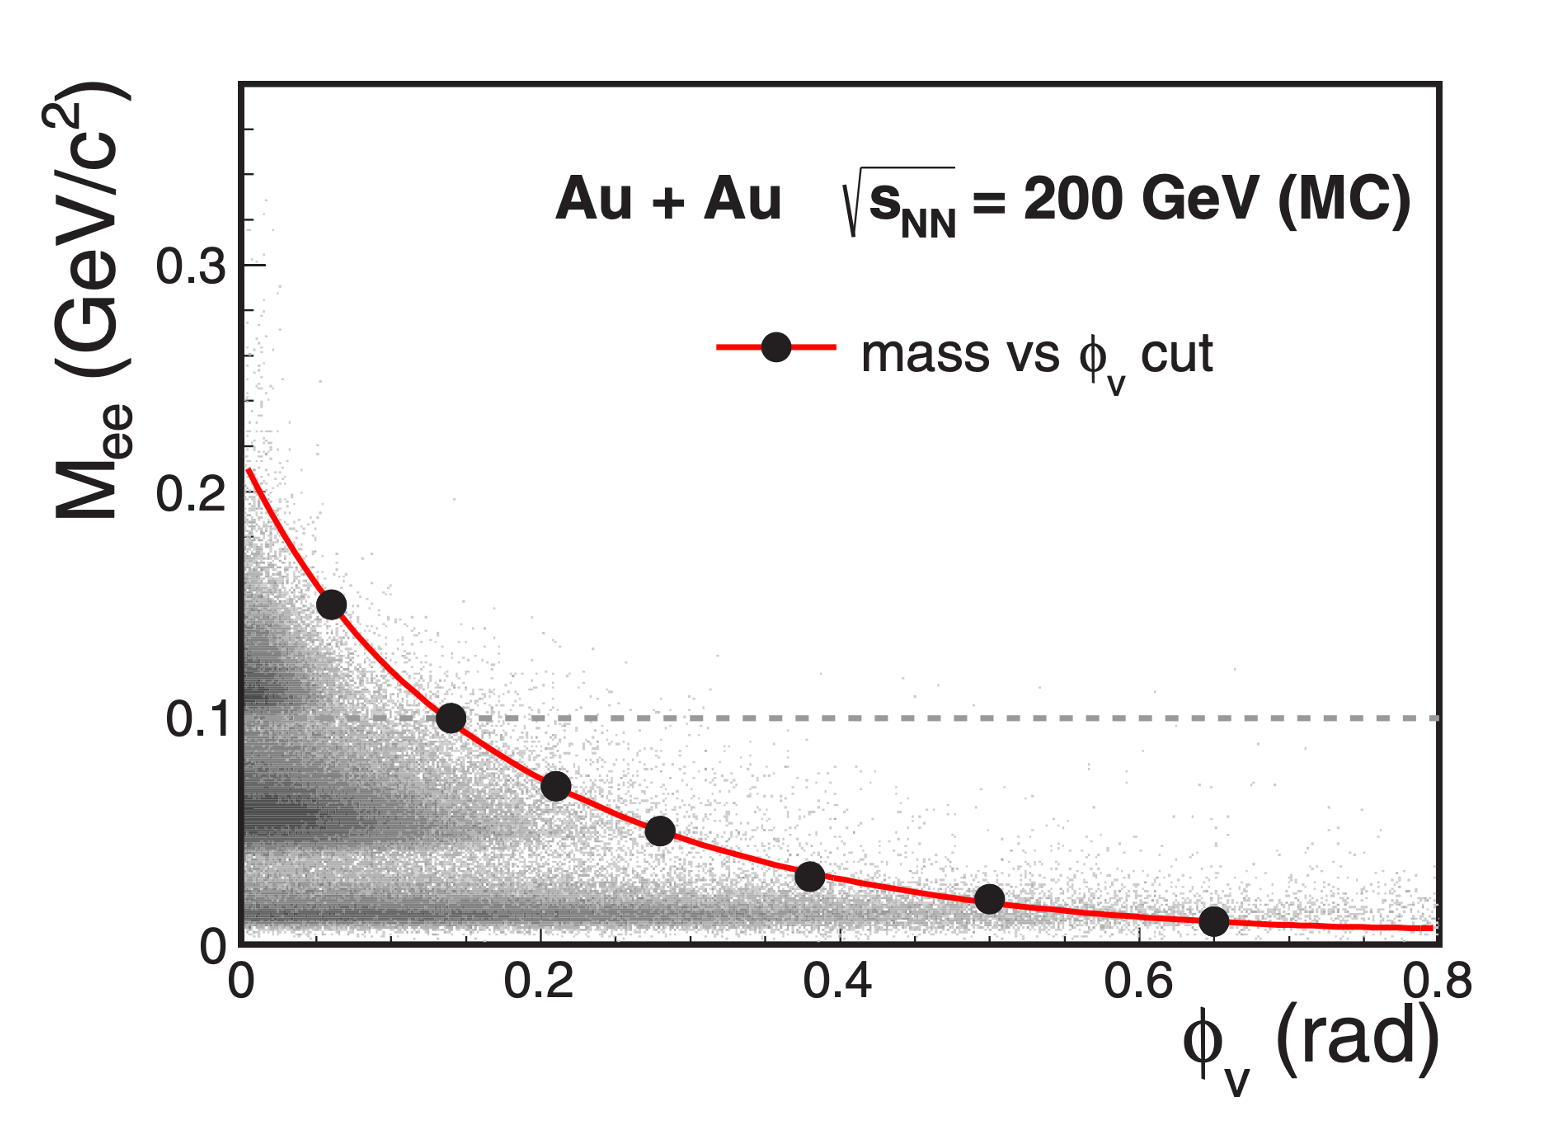
\includegraphics[width=0.75\textwidth,clip]{figures/Chapter4/PhiV.png}
  \end{center}
  \caption[\sNN = 200 GeV金-金对撞中模拟得到的 \PhiV 分布示意图]{\sNN = 200 GeV金-金对撞中GEANT模拟得到的 \PhiV 分布示意图}
  \label{c}
\end{figure}

\subsection{原初信号}
在应用了 \PhiV 判选条件的 \Npm 分布中进行背景扣除即可得到原初信号(raw signal)。之所以被称为原初信号是因为在此时,双电子谱并未经过效率和探测器接收度的修正,无法与其他实验甚至STAR其他能量的结果进行比较。在经过效率修正以后的结果即为在STAR接收度下一定快度区间没有效率损失的双电子谱。而由于不同探测器的接收度不同,经过效率修正的电子谱需要再经过探测器接收度修正,得到全接收度的双电子谱后才可以和其他实验接收度修正后的谱进行比较。关于效率修正和探测器接收度修正的部分将在 \ref{chap:pair_eff}和\ref{chap:pair_acc}小节当中讨论。